\documentclass[10pt,a4paper]{article}

\usepackage[margin=0.78in]{geometry}
\usepackage[T1]{fontenc}
\usepackage[utf8]{inputenc}
\usepackage{lmodern}
\usepackage{microtype}
\usepackage{parskip}
\usepackage{enumitem}
\usepackage{booktabs}
\usepackage{tabularx}
\usepackage{array}
\usepackage{xcolor}
\usepackage{tikz}
\usetikzlibrary{positioning}
\usepackage[most]{tcolorbox}
\usepackage{titlesec}
\usepackage[hidelinks]{hyperref}
\usepackage{fancyhdr}

\definecolor{navy}{HTML}{19466F}
\definecolor{deepnavy}{HTML}{123653}
\definecolor{pale}{HTML}{EAF2FB}
\definecolor{green}{HTML}{2E7D32}
\definecolor{greenpale}{HTML}{EDF8EE}
\definecolor{amber}{HTML}{9A6700}
\definecolor{amberpale}{HTML}{FFF6D8}
\definecolor{red}{HTML}{9F2D20}
\definecolor{redpale}{HTML}{FCEDEA}
\definecolor{graybox}{HTML}{F3F5F7}
\definecolor{midgray}{HTML}{5F6B75}

\hypersetup{
  pdftitle={Collaborative Inference at the Edge: A Beginner's Guide},
  pdfauthor={Study companion},
  pdfsubject={Beginner introduction to HexGen, Jupiter, CI-Inf, and FOCI}
}

\titleformat{\section}{\Large\bfseries\color{navy}}{\thesection}{0.7em}{}
\titleformat{\subsection}{\large\bfseries\color{navy}}{\thesubsection}{0.65em}{}
\titlespacing*{\section}{0pt}{1.2em}{0.45em}
\titlespacing*{\subsection}{0pt}{0.9em}{0.35em}

\setlist[itemize]{leftmargin=1.45em,itemsep=0.25em,topsep=0.35em}
\setlist[enumerate]{leftmargin=1.55em,itemsep=0.25em,topsep=0.35em}
\renewcommand{\arraystretch}{1.18}
\setlength{\emergencystretch}{2em}

\pagestyle{fancy}
\fancyhf{}
\fancyhead[L]{\small\color{midgray}Collaborative Inference: Beginner's Guide}
\fancyfoot[C]{\thepage}
\renewcommand{\headrulewidth}{0.2pt}

\newtcolorbox{takeaway}[1][One-sentence takeaway]{
  enhanced, breakable, colback=pale, colframe=navy, boxrule=0.7pt,
  arc=2pt, left=8pt,right=8pt,top=5pt,bottom=5pt,
  title={#1}, colbacktitle=navy, coltitle=white, fonttitle=\bfseries
}
\newtcolorbox{plainbox}[1][In plain language]{
  enhanced, breakable, colback=graybox, colframe=deepnavy, boxrule=0.7pt,
  arc=2pt, left=8pt,right=8pt,top=5pt,bottom=5pt,
  title={#1}, colbacktitle=deepnavy, coltitle=white, fonttitle=\bfseries
}
\newtcolorbox{resultbox}[1][What the evaluation found]{
  enhanced, breakable, colback=greenpale, colframe=green, boxrule=0.7pt,
  arc=2pt, left=8pt,right=8pt,top=5pt,bottom=5pt,
  title={#1}, colbacktitle=green, coltitle=white, fonttitle=\bfseries
}
\newtcolorbox{cautionbox}[1][Do not overgeneralize]{
  enhanced, breakable, colback=amberpale, colframe=amber, boxrule=0.7pt,
  arc=2pt, left=8pt,right=8pt,top=5pt,bottom=5pt,
  title={#1}, colbacktitle=amber, coltitle=white, fonttitle=\bfseries
}
\newtcolorbox{checkbox}[1][Quick check]{
  enhanced, breakable, colback=redpale, colframe=red, boxrule=0.7pt,
  arc=2pt, left=8pt,right=8pt,top=5pt,bottom=5pt,
  title={#1}, colbacktitle=red, coltitle=white, fonttitle=\bfseries
}

\newcommand{\term}[1]{\textbf{\color{navy}#1}}
\newcommand{\paper}[1]{\textit{#1}}

\begin{document}

\begin{titlepage}
\thispagestyle{empty}
\centering
\vspace*{2.1cm}
{\fontsize{29}{35}\selectfont\bfseries\color{navy}Collaborative Inference at the Edge\par}
\vspace{0.45cm}
{\Large\color{navy}LLMs, heterogeneous devices, and fair resource sharing\par}
\vspace{1.0cm}
{\large A beginner's guide to four selected papers\par}
\vspace{0.45cm}
{\large HexGen \quad $\bullet$ \quad Jupiter \quad $\bullet$ \quad CI-Inf Poster \quad $\bullet$ \quad FOCI\par}

\vspace{1.3cm}
\begin{tcolorbox}[width=0.82\textwidth,colback=graybox,colframe=navy,boxrule=0.9pt,arc=3pt]
\centering
This guide assumes no prior knowledge of LLM serving or edge computing. It explains the minimum background first, then separates two related questions:

\vspace{0.25em}
\textbf{How can several machines run one large model?}\quad and\quad
\textbf{How should many users fairly share edge resources?}
\end{tcolorbox}

\vfill
{\large Prepared as a study companion\par}
\vspace{0.25cm}
{\large Reviewed edition --- July 2026\par}
\end{titlepage}

\tableofcontents

\section*{How to use this guide}
\addcontentsline{toc}{section}{How to use this guide}

The papers are connected, but they do \emph{not} all solve the same problem. HexGen, Jupiter, and the FSU CI-Inf poster divide one LLM across multiple machines. FOCI instead studies many mobile devices that each run or offload a DNN inference job while sharing edge servers. FOCI is included because it exposes the next coordination problem: once collaboration becomes multi-user and mobile, speed alone is not enough; fairness and stable decisions matter too.

For a first reading:
\begin{enumerate}
  \item Read Sections 1--2 for vocabulary.
  \item Read the blue takeaway and green evaluation boxes for each paper.
  \item Return to the detailed paragraphs when you need to explain \emph{why} a method works.
\end{enumerate}

\begin{cautionbox}[Scope of this document]
This is a guide to four selected references, not a survey of every PDF in the folder. Reported speedups are results from each paper's particular models, devices, networks, and baselines; they are not universal performance guarantees.
\end{cautionbox}

\part*{Part I --- Background}
\addcontentsline{toc}{part}{Part I --- Background}

\section{What an LLM does during inference}

A decoder-only LLM, such as Llama, is a stack of transformer layers. Text is divided into \term{tokens}, and each token is represented by a vector called a \term{hidden state} or \term{activation}. That representation passes through every layer. At the end, the model assigns scores to possible next tokens.

Two facts motivate distributed inference:
\begin{enumerate}
  \item \textbf{The model can be too large for one device.} For example, 70 billion parameters require about 140 GB just for weights at 16-bit precision, before temporary activations and caches.
  \item \textbf{Text generation is sequential.} After the prompt is processed, output token $t+1$ depends on the tokens already generated through $t$.
\end{enumerate}

\subsection{Prefill and decoding}

\begin{takeaway}
\textbf{Prefill} reads the prompt; \textbf{decoding} generates the answer one token at a time. They stress hardware differently, so a system may need a different optimization for each phase.
\end{takeaway}

During \term{prefill}, the model processes all prompt tokens and constructs the internal history needed for generation. Prefill usually contains large matrix operations and can be compute-intensive. During \term{decoding}, the model produces one token per iteration. Each iteration performs relatively little arithmetic but repeatedly reads model weights and the stored history, making decoding sensitive to memory bandwidth and communication delay.

Which phase dominates depends on prompt length, output length, batch size, and hardware. Long prompts can make prefill expensive; long answers often make decoding dominate total latency.

\subsection{The KV cache}

In every attention layer, a token is transformed into query, key, and value vectors. Earlier keys and values are reused when later tokens are generated. The \term{KV cache} stores those reusable keys and values, avoiding repeated computation of the entire history.

\begin{plainbox}
The KV cache is the model's fast working memory for attention. It grows as the prompt and answer grow. It can become a major memory cost for long contexts or large batches, but it does \textbf{not automatically exceed the model weights} in every workload.
\end{plainbox}

Both weights and the KV cache matter in the FSU poster: distributing layers also distributes the weights and the corresponding per-layer cache.

\subsection{The memory wall}

If weights, the KV cache, and working tensors do not fit in fast accelerator memory, a system may move some data to CPU memory. That makes capacity larger, but repeated CPU--GPU transfers can slow generation. This capacity-versus-speed conflict is often called a \term{memory wall}.

\section{How one model can be divided across machines}

\subsection{Tensor parallelism}

\term{Tensor parallelism (TP)} divides the matrix operations inside each layer across devices. Devices work on the same layer at the same time, then combine partial results using collective communication such as all-reduce. Common transformer TP designs synchronize around the attention and feed-forward portions of each layer.

TP can reduce computation latency when devices have very fast links. On ordinary Ethernet, Wi-Fi, or wide-area connections, frequent synchronization can dominate.

\subsection{Pipeline parallelism}

\term{Pipeline parallelism (PP)} gives each device a consecutive block of complete layers, called a stage. A request passes through stage 1, then stage 2, and so on. Communication occurs mainly at stage boundaries.

During decoding, a boundary message for one sequence is approximately one token's hidden-state vector. During prefill or batching, it is a larger activation tensor containing multiple tokens or requests. It is still usually much less frequent than layer-by-layer TP synchronization, but it should not always be described as ``one tiny vector.''

\begin{center}
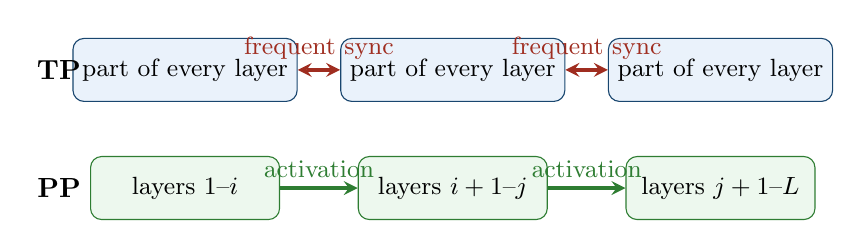
\begin{tikzpicture}[font=\small,>=stealth]
  \node[draw=navy,rounded corners,fill=pale,minimum width=2.4cm,minimum height=0.8cm] (t1) at (0,1.5) {part of every layer};
  \node[draw=navy,rounded corners,fill=pale,minimum width=2.4cm,minimum height=0.8cm] (t2) at (3.4,1.5) {part of every layer};
  \node[draw=navy,rounded corners,fill=pale,minimum width=2.4cm,minimum height=0.8cm] (t3) at (6.8,1.5) {part of every layer};
  \draw[<->,very thick,red] (t1) -- node[above]{frequent sync} (t2);
  \draw[<->,very thick,red] (t2) -- node[above]{frequent sync} (t3);
  \node[anchor=east,font=\bfseries] at (-1.2,1.5) {TP};

  \node[draw=green,rounded corners,fill=greenpale,minimum width=2.4cm,minimum height=0.8cm] (p1) at (0,0) {layers 1--$i$};
  \node[draw=green,rounded corners,fill=greenpale,minimum width=2.4cm,minimum height=0.8cm] (p2) at (3.4,0) {layers $i+1$--$j$};
  \node[draw=green,rounded corners,fill=greenpale,minimum width=2.4cm,minimum height=0.8cm] (p3) at (6.8,0) {layers $j+1$--$L$};
  \draw[->,very thick,green] (p1) -- node[above]{activation} (p2);
  \draw[->,very thick,green] (p2) -- node[above]{activation} (p3);
  \node[anchor=east,font=\bfseries] at (-1.2,0) {PP};
\end{tikzpicture}
\end{center}

\begin{cautionbox}[The trade-off, not a universal winner]
TP is usually attractive on tightly connected GPUs; PP is often attractive across slower links and when model memory must be distributed. PP can nevertheless leave stages idle for a single request. Jupiter is largely about recovering that lost parallelism.
\end{cautionbox}

\subsection{Sequence parallelism and speculative decoding}

\term{Sequence parallelism (SP)} divides tokens across devices, but transformer attention often requires synchronization of information across those tokens. \term{Speculative decoding} instead guesses several future tokens using a cheaper draft mechanism and verifies them with the target model, reducing the number of expensive decoding iterations when guesses are accepted.

\subsection{Why heterogeneity is difficult}

A homogeneous cluster has similar devices and links. A heterogeneous cluster may mix strong and weak accelerators, different memory capacities, and links ranging from fast local interconnects to slow wide-area networks. Equal partitions then create bottlenecks: the slowest stage determines pipeline throughput, and one infeasible memory assignment can prevent deployment.

\begin{plainbox}
Think of a relay team whose runners have different speeds and whose handoff zones have different lengths. Equal segments are not fair or fast. The schedule must account for both the runner and the handoff.
\end{plainbox}

\part*{Part II --- Four selected papers}
\addcontentsline{toc}{part}{Part II --- Four selected papers}

\section{HexGen: heterogeneous LLM serving across datacenters}

\textit{Jiang et al., ICML 2024.}

\begin{takeaway}
HexGen assigns unequal model portions and unequal tensor-parallel widths to unequal GPUs, then searches for a layout that respects memory, compute, and network constraints.
\end{takeaway}

\subsection{Problem}

Large LLMs are commonly served on identical high-end GPUs in one datacenter. HexGen asks whether a mixed, geographically distributed GPU pool can provide competitive service at lower cost. Standard symmetric layouts waste heterogeneous resources because they expect stages to contain equal layer counts or use the same TP degree.

\subsection{Core idea: asymmetric hybrid parallelism}

HexGen allows pipeline stages to differ. One stage may contain more layers or use more GPUs than another. In general, it favors TP among GPUs with fast local links and PP across slower machine or regional boundaries. A designated leader handles communication between TP groups, limiting cross-group transfers.

\subsection{How the layout is chosen}

The scheduler models three costs: computation, communication, and memory. It uses dynamic programming to select stage configurations inside a candidate group and a genetic search to modify the global grouping through merge, split, and swap operations. The search is a practical approximation to a hard combinatorial placement problem.

\begin{resultbox}
For Llama-2-70B, HexGen reports up to \textbf{2.3$\times$ lower latency deadlines} or support for up to \textbf{4$\times$ higher request rates} than a homogeneous deployment at a similar hourly budget. After four GPUs leave, its local-search-based replanning completes in under 30 seconds in the reported experiment.
\end{resultbox}

\begin{cautionbox}[What HexGen does not yet solve]
The evaluated implementation lacks advanced heterogeneous batching. Its planner primarily treats transformer execution as dense, and its main objective is service cost/performance rather than energy, privacy, or fairness.
\end{cautionbox}

\section{Jupiter: collaborative LLM inference on edge devices}

\textit{Ye et al., IEEE INFOCOM 2025.}

\begin{takeaway}
Jupiter makes pipeline parallelism useful for a single request by pipelining chunks of the prompt and by exposing additional parallelism during decoding.
\end{takeaway}

\subsection{Problem}

Jupiter targets nearby resource-limited devices, such as Jetson boards on a local network. TP and SP communicate frequently, while ordinary PP processes a single request stage by stage and leaves other devices idle. Earlier collaborative edge systems also concentrated mainly on prefill, even though decoding may dominate long responses.

\subsection{Intra-sequence pipeline parallelism}

Causal attention means a token attends only to itself and earlier tokens. Jupiter divides a prompt into consecutive subsequences and injects them into the layer pipeline. Each stage caches earlier hidden states so a later subsequence can attend to all preceding subsequences correctly.

The planner chooses:
\begin{itemize}
  \item how many consecutive layers each device receives; and
  \item how long each prompt chunk should be.
\end{itemize}

Chunks are not necessarily equal because later chunks attend to more history and can require more work.

\subsection{Decoding acceleration}

Jupiter adds two mechanisms:
\begin{itemize}
  \item \textbf{Self-speculative decoding:} lightweight heads draft candidate tokens; the full model verifies candidates and removes rejected candidates from each stage's KV cache.
  \item \textbf{Outline-based parallel decoding:} the model first creates an outline, then expands different points as separate requests through the pipeline.
\end{itemize}

The outline mechanism is optional. It works for separable sections but can reduce quality on tasks with strict sequential dependencies, especially mathematics and coding. Standard speculative verification is designed to preserve the target model's decoding behavior; outline decomposition intentionally changes the generation procedure and is therefore not lossless.

\begin{resultbox}
On the paper's Jetson testbeds and INT4 Llama-2 models, Jupiter reports up to \textbf{26.1$\times$ lower end-to-end latency} than the most communication-heavy baselines and up to \textbf{2.7$\times$} improvement over a serial pipeline. Its two decoding mechanisms together reach up to \textbf{3.9$\times$} speedup over naive sequential generation.
\end{resultbox}

\begin{cautionbox}[How to interpret the headline]
The 26.1$\times$ figure is a maximum across particular baselines, bandwidths, models, and device configurations. Jupiter is not 26.1$\times$ faster than every distributed system in every setting.
\end{cautionbox}

\clearpage
\section{The FSU CI-Inf poster: a real three-device pipeline}

\textit{Zhou and Zhang, HotMobile 2026 poster / one-page extended abstract.}

\begin{takeaway}
CI-Inf divides Llama-3.2-3B by complete layers across three Jetson Orin Nano devices, keeping each stage's weights and KV cache in local fast memory and avoiding repeated CPU--GPU swapping.
\end{takeaway}

The poster is intentionally smaller in scope than HexGen or Jupiter. It demonstrates one clean design on real hardware rather than proposing a complete scheduler.

\subsection{Baseline problem: one device under memory pressure}

The single-device baseline uses CPU/GPU memory sharing because the complete workload cannot remain in GPU memory. During autoregressive decoding, repeated movement between CPU and GPU adds substantial per-token time.

\begin{plainbox}
The problem is not that the GPU cannot perform the arithmetic. It is that the model state cannot all remain in the GPU's fast memory, so computation repeatedly waits for data movement.
\end{plainbox}

\subsection{Prototype design}

The 28 decoder layers are placed as follows:

\begin{center}
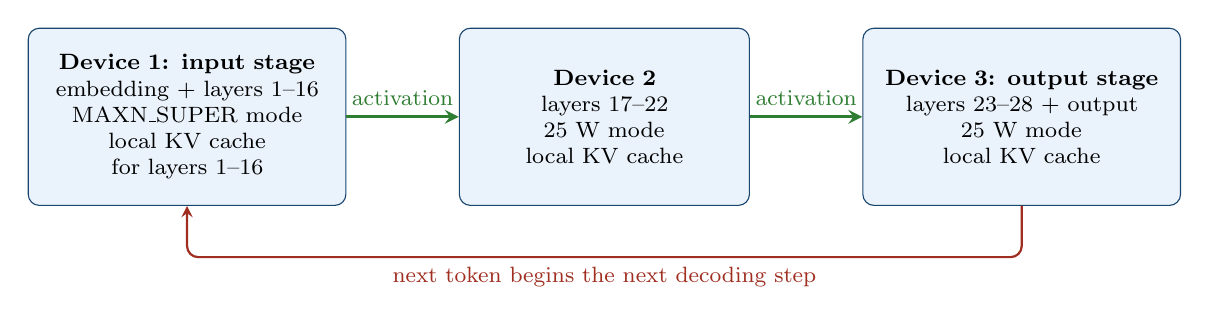
\begin{tikzpicture}[font=\footnotesize,>=stealth]
  \node[draw=navy,rounded corners,fill=pale,text width=3.8cm,minimum height=2.25cm,align=center] (d1) at (0,0) {
    \textbf{Device 1: input stage}\\
    embedding + layers 1--16\\
    MAXN\_SUPER mode\\
    local KV cache for layers 1--16};
  \node[draw=navy,rounded corners,fill=pale,text width=3.45cm,minimum height=2.25cm,align=center] (d2) at (5.3,0) {
    \textbf{Device 2}\\
    layers 17--22\\
    25 W mode\\
    local KV cache};
  \node[draw=navy,rounded corners,fill=pale,text width=3.8cm,minimum height=2.25cm,align=center] (d3) at (10.6,0) {
    \textbf{Device 3: output stage}\\
    layers 23--28 + output\\
    25 W mode\\
    local KV cache};
  \draw[->,very thick,green] (d1.east) -- node[above]{activation} (d2.west);
  \draw[->,very thick,green] (d2.east) -- node[above]{activation} (d3.west);
  \draw[->,thick,red,rounded corners] (d3.south) -- ++(0,-0.65) -- node[below]{next token begins the next decoding step} ++(-10.6,0) -- (d1.south);
\end{tikzpicture}

\small Inter-stage transfers use 1 Gbps Ethernet.
\end{center}

\textbf{1. Complete-layer ownership.} Each device owns a consecutive group of decoder layers. It performs all operations in those layers before sending the resulting activation to the next stage.

\textbf{2. Distributed memory.} Each device stores only its layers' weights and KV cache. The aggregate memory of the three devices is used without repeatedly swapping every layer through one device's CPU memory.

\textbf{3. Boundary communication.} Only inter-stage activations and the decoding-loop control information cross devices. This is less frequent than a conventional layer-wise TP collective, although communication still adds measurable latency.

\textbf{4. Unequal placement.} The reported 16/6/6 placement corresponds to unequal power modes and stage responsibilities. The poster demonstrates this placement; it does not claim a general optimizer proved it globally optimal.

\clearpage
\subsection{Experiment and interpretation}

\begin{center}
\begin{tabularx}{0.92\textwidth}{>{\bfseries}lXX}
\toprule
 & Single-device baseline & CI-Inf pipeline \\
\midrule
Hardware & One device using CPU/GPU memory sharing & Three Jetson Orin Nanos over 1 Gbps Ethernet \\
Model & \multicolumn{2}{l}{Llama-3.2-3B-Instruct, bf16, 28 decoder layers} \\
Total elapsed time & 32,213.9 ms & 18,989.8 ms \\
Average token time & 325.39 ms & 191.82 ms \\
\bottomrule
\end{tabularx}
\end{center}

The pipeline reduces total elapsed time by about 40\%. Its mean token time consists of approximately 157.31 ms of computation across the three stages plus 34.51 ms of communication. The network overhead is real, but it is smaller than the time avoided by eliminating the baseline's repeated memory movement.

\begin{cautionbox}[What the poster establishes --- and what it does not]
It establishes feasibility and a useful speed improvement on one three-device prototype. As a one-page poster, it does not yet establish optimal partitioning, scaling to many devices, behavior under Wi-Fi or device failures, quality effects, energy savings, or superiority over optimized distributed frameworks such as Jupiter.
\end{cautionbox}

\section{FOCI: fair collaborative inference for mobile users}

\textit{Zhou and Zhang, NeurIPS 2025 AI4NextG Workshop.}

\begin{takeaway}
FOCI uses multi-agent reinforcement learning to help moving devices choose an edge server and model split while protecting the worst-served user's latency and energy performance.
\end{takeaway}

\subsection{Why this paper is different}

FOCI is not primarily an LLM-serving paper. Its experiment uses MobileNetV3-large and studies many devices, each with its own inference workload. A device chooses:
\begin{itemize}
  \item whether and where to offload computation; and
  \item where to split its DNN between local and edge execution.
\end{itemize}

If many devices choose the same edge, they compete for limited streaming multiprocessors. Mobility changes channel conditions and the competitor set. The objective is \term{max--min fairness}: improve the worst device rather than only optimizing the average.

\subsection{Two components}

\textbf{Fairness-oracle reward shaping.} Each edge solves a local max--min resource-allocation problem for its connected devices. It returns this fairness-aligned signal during training. The paper uses a continuous relaxation followed by a min-risk rounding/search procedure to keep this calculation practical.

\textbf{Competitor-aware observation augmentation.} Basic mean-field MARL summarizes the behavior of other agents. A geographic-neighbor summary changes rapidly as devices move; a global summary includes many irrelevant devices. FOCI instead collects anonymous aggregate action records from edges inside a perception domain that could plausibly contend with the target device.

\begin{plainbox}
FOCI does not tell a device exactly what every neighbor is doing. It provides a compact distribution of relevant recent actions. This improves scalability and reveals less individual information, although the paper does not provide a formal differential-privacy guarantee.
\end{plainbox}

\subsection{Theory and results}

FOCI bounds the difference between Q-values computed from its sampled aggregate action distribution and those based on the global distribution, then derives a bounded gap from a Nash-equilibrium Q-value under stated assumptions.

\begin{cautionbox}[Correct interpretation of the paper's $\lambda$]
The theorem uses $\lambda$ for the expected number of nonzero dimensions in the sampled action distribution. In the displayed bound, smaller $\lambda$ by itself makes the bound looser, not tighter. Therefore, it is inaccurate to say that ``more sparsity automatically tightens the guarantee.'' FOCI's practical benefit comes from selecting a more relevant and stable summary; the theorem also rewards adequate coverage of that summary.
\end{cautionbox}

\begin{resultbox}
In simulation with 240 devices, 11 edges, Porto taxi trajectories, Jetson TX2 profiles, and MobileNetV3-large, FOCI reports up to \textbf{56\% lower worst-case latency} and \textbf{46\% lower worst-case energy} than baselines, while roughly halving switching cost relative to the compared RL methods.
\end{resultbox}

\section{How the four papers fit together}

\begin{tabularx}{\textwidth}{>{\bfseries}p{1.6cm}p{2.5cm}p{2.6cm}X}
\toprule
Paper & Setting & Main objective & Signature idea \\
\midrule
HexGen & Mixed GPUs across regions & Cost, SLO attainment, request rate & Asymmetric hybrid TP/PP plus placement search \\
Jupiter & Small edge-device cluster & Prefill and decoding latency & Intra-sequence pipeline plus speculative/outline decoding \\
CI-Inf & Three-device edge prototype & Avoid memory swapping; reduce token latency & Complete-layer placement with local per-stage KV caches \\
FOCI & Moving devices sharing edges & Worst-device fairness and stable choices & Fairness oracle plus competitor-aware mean field \\
\bottomrule
\end{tabularx}

\subsection{A useful mental model}

The first three papers answer \textbf{placement}: where should the model's computation and memory live? FOCI answers \textbf{coordination}: when many decision makers share edge resources, how should their choices account for one another?

Together they suggest a future end-to-end system with three layers:
\begin{enumerate}
  \item \textbf{Representation layer:} decide what information really needs to be stored or transmitted.
  \item \textbf{Systems layer:} place model components across heterogeneous devices.
  \item \textbf{Control layer:} adapt placement and sharing decisions as workloads, links, and users change.
\end{enumerate}

\begin{takeaway}[Connection to high-dimensional data and sparsity]
All three LLM systems still plan mostly around dense weights, activations, and KV-cache blocks. A natural research direction is to represent stage-boundary activations or caches using structured sparsity or low-rank-plus-sparse tensors, then co-design compression with device placement. The important question is not simply ``can zeros be removed?'' but ``does the compressed structure produce real end-to-end speedups after indexing, reconstruction, and sparse-kernel overhead?''
\end{takeaway}

\section{Common misconceptions}

\begin{enumerate}
  \item \textbf{``Pipeline parallelism is always faster.''} No. It reduces communication frequency but may create idle stages and is limited by the slowest stage.
  \item \textbf{``The KV cache is always larger than the weights.''} No. It depends on model architecture, precision, context length, and batch size.
  \item \textbf{``Speculative decoding and outline decoding are both lossless.''} No. Verification-based speculation can preserve the target distribution; outline decomposition changes how an answer is generated and can reduce reasoning quality.
  \item \textbf{``FOCI distributes one LLM across devices.''} No. FOCI coordinates many mobile DNN-inference users sharing edge servers.
  \item \textbf{``Anonymous aggregates prove privacy.''} No. They reduce direct telemetry exposure, but formal privacy requires an explicit threat model and guarantee.
  \item \textbf{``A maximum speedup applies everywhere.''} No. Always check model, precision, devices, network, prompt/output lengths, and baseline.
\end{enumerate}

\section{Glossary}

\begin{description}[style=nextline,leftmargin=0pt,labelwidth=0pt,labelsep=0pt,labelindent=0pt]
  \item[\term{Activation / hidden state}] Numeric representation passed between layers or pipeline stages.
  \item[\term{All-reduce}] Collective operation that combines partial tensors from multiple devices.
  \item[\term{Autoregressive decoding}] Generation in which each new token depends on earlier tokens.
  \item[\term{Causal attention}] Attention rule that prevents a token from using future tokens.
  \item[\term{Decoding}] Token-by-token answer generation after prefill.
  \item[\term{Edge device / edge server}] A user-side or nearby device / a nearby shared compute node.
  \item[\term{Heterogeneous}] Composed of devices or links with different capabilities.
  \item[\term{KV cache}] Stored attention keys and values for previous tokens at every layer.
  \item[\term{Max--min fairness}] Optimize the outcome of the worst-served participant.
  \item[\term{Mean-field MARL}] Multi-agent learning in which each agent observes an aggregate of other behavior.
  \item[\term{Memory wall}] Performance limit caused by insufficient fast memory or excessive data movement.
  \item[\term{Pipeline bubble}] Idle time while a stage waits for work or for another stage to finish.
  \item[\term{Pipeline parallelism}] Put consecutive complete layers on different devices.
  \item[\term{Prefill}] Process the complete input prompt and construct the initial KV cache.
  \item[\term{Speculative decoding}] Draft several future tokens cheaply and verify them with the target model.
  \item[\term{Tensor parallelism}] Divide the operations inside each layer across devices.
  \item[\term{Token}] A text unit processed by an LLM; it may be a word, word piece, or symbol.
\end{description}

\section*{Selected references}
\addcontentsline{toc}{section}{Selected references}

\begin{enumerate}
  \item Y. Jiang et al. \paper{HexGen: Generative Inference of Large Language Model over Heterogeneous Environment}. ICML, 2024.
  \item S. Ye et al. \paper{Jupiter: Fast and Resource-Efficient Collaborative Inference of Generative LLMs on Edge Devices}. IEEE INFOCOM, 2025.
  \item H. Zhou and X. Zhang. \paper{Poster: Distributed Pipelined Collaborative Inference for LLMs on Edge Device Clusters}. HotMobile, 2026.
  \item H. Zhou and X. Zhang. \paper{Fairness-Oracular MARL with Competitor-Aware Signals for Collaborative Inference}. NeurIPS AI4NextG Workshop, 2025.
\end{enumerate}

\begin{checkbox}[Three questions to test your understanding]
\begin{enumerate}
  \item Why can PP be better than TP on ordinary Ethernet even if TP exposes more arithmetic parallelism?
  \item How does Jupiter use causal attention to fill a pipeline during prefill?
  \item Why is FOCI's fairness problem different from HexGen's placement problem?
\end{enumerate}
\end{checkbox}

\end{document}
